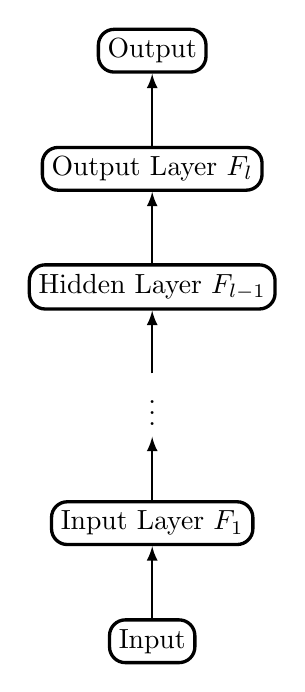
\begin{tikzpicture}[
	cell/.style={
		rectangle, 
		rounded corners=2mm, 
		draw,
		very thick,
		align=center,
	},
	ArrowC1/.style={% Arrows with rounded corners
		rounded corners=.25cm,
		thick,
	},
]
	\node [cell] (out) at (0,7.5) {Output};
	\node [cell] (fl) at (0,6) {Output Layer $F_l$};
	\node [cell] (fl1) at (0,4.5) {Hidden Layer $F_{l-1}$};
	\node [very thick, align = center](dots) at (0,3) {\vdots};
	\node [cell] (f1) at (0,1.5) {Input Layer $F_1$};
	\node [cell] (in) at (0,0) {Input};
	
	\draw [-latex,ArrowC1] (fl) -- (out);
	\draw [-latex,ArrowC1] (fl1) -- (fl);
	\draw [-latex,ArrowC1] (dots) -- (fl1);
	\draw [-latex,ArrowC1] (f1) -- (dots);
	\draw [-latex,ArrowC1] (in) -- (f1);
\end{tikzpicture}